\documentclass[11pt,a4paper]{article}

% ====================================================================
% Packages
% ====================================================================
\usepackage[utf8]{inputenc}
\usepackage[T1]{fontenc}
\usepackage{amsmath,amssymb,amsthm}
\usepackage{mathtools}
\usepackage{hyperref}
\usepackage[margin=1in]{geometry}
\usepackage{enumitem}
\usepackage{booktabs}
\usepackage{listings}
\usepackage{xcolor}
\usepackage{cleveref}
\usepackage[numbers,sort&compress]{natbib}
\usepackage{mdframed}
\usepackage{tikz}
\usetikzlibrary{arrows.meta,positioning}

% ====================================================================
% Theorem environments
% ====================================================================
\theoremstyle{plain}
\newtheorem{theorem}{Theorem}[section]
\newtheorem{lemma}[theorem]{Lemma}
\newtheorem{proposition}[theorem]{Proposition}
\newtheorem{corollary}[theorem]{Corollary}

\theoremstyle{definition}
\newtheorem{definition}[theorem]{Definition}
\newtheorem{remark}[theorem]{Remark}

% ====================================================================
% Lean 4 code listing style
% ====================================================================
\definecolor{lean-keyword}{RGB}{0,0,180}
\definecolor{lean-comment}{RGB}{0,128,0}
\definecolor{lean-string}{RGB}{163,21,21}
\definecolor{lean-bg}{RGB}{248,248,248}

\lstdefinelanguage{lean4}{
  keywords={theorem,lemma,def,class,instance,import,open,variable,
            noncomputable,section,namespace,end,where,let,have,show,
            intro,obtain,use,exact,rw,simp,apply,by,fun,match,if,
            then,else,do,return,axiom,abbrev,private,attribute,
            suffices,change,congr,ext,constructor,rintro,push_neg,
            linarith,absurd,set_option,omit,in,set,cases,left,right,
            nlinarith,push_cast,positivity,omega,refine,field_simp,
            structure,calc,ring,fun_prop,unfold,induction,deriving,
            inductive,rcases},
  sensitive=true,
  morecomment=[l]{--},
  morecomment=[s]{/-}{-/},
  morestring=[b]",
  morestring=[b]',
}

\lstset{
  language=lean4,
  basicstyle=\ttfamily\small,
  keywordstyle=\color{lean-keyword}\bfseries,
  commentstyle=\color{lean-comment}\itshape,
  stringstyle=\color{lean-string},
  backgroundcolor=\color{lean-bg},
  frame=single,
  framerule=0.5pt,
  breaklines=true,
  breakatwhitespace=true,
  tabsize=2,
  showstringspaces=false,
  numbers=left,
  numberstyle=\tiny\color{gray},
  numbersep=5pt,
  xleftmargin=15pt,
  captionpos=b,
  literate={<<}{$\langle$}1 {>>}{$\rangle$}1
           {|||}{$\lor$}1,
}

% ====================================================================
% Macros
% ====================================================================
\newcommand{\NN}{\mathbb{N}}
\newcommand{\RR}{\mathbb{R}}
\newcommand{\ZZ}{\mathbb{Z}}
\newcommand{\QQ}{\mathbb{Q}}
\newcommand{\LPO}{\ensuremath{\mathrm{LPO}}}
\newcommand{\WLPO}{\ensuremath{\mathrm{WLPO}}}
\newcommand{\LLPO}{\ensuremath{\mathrm{LLPO}}}
\newcommand{\BMC}{\ensuremath{\mathrm{BMC}}}
\newcommand{\BISH}{\ensuremath{\mathrm{BISH}}}
\newcommand{\MP}{\ensuremath{\mathrm{MP}}}
\newcommand{\CPgW}{\ensuremath{\mathrm{CPgW}}}
\newcommand{\Lean}{\textsc{Lean~4}}
\newcommand{\Mathlib}{\textsc{Mathlib4}}
\newcommand{\leanok}{\textsf{\small \textcolor{green!70!black}{\checkmark}}}
\newcommand{\leanaxiom}{\textsf{\small \textcolor{orange!80!black}{(axiom)}}}

% ====================================================================
% Title
% ====================================================================
\title{%
  \textbf{Stratifying Spectral Gap Undecidability}\\[6pt]
  {\normalsize Cubitt's Theorem Is $\LPO$: Macroscopic Quantum Undecidability
  Costs Exactly One Thermodynamic Limit}\\[6pt]
  {\normalsize A Lean~4 Formalization (Paper~36)}%
}

\author{
  Paul Chun-Kit Lee\thanks{%
    New York University.
    AI-assisted formalization; see \S\ref{sec:ai} for methodology.} \\
  New York University \\
  \texttt{dr.paul.c.lee@gmail.com}
}

\date{February 14, 2026\\[4pt]
  {\small DOI: \href{https://doi.org/10.5281/zenodo.18642620}{10.5281/zenodo.18642620}}}

% ====================================================================
\begin{document}
\maketitle

% ====================================================================
\begin{abstract}
Cubitt, Perez-Garcia, and Wolf proved that the spectral gap problem
is undecidable: no algorithm determines whether an arbitrary
translation-invariant Hamiltonian is gapped or gapless in the
thermodynamic limit. We prove that this undecidability is
Turing--Weihrauch equivalent\footnote{Throughout, ``Turing--Weihrauch
equivalent'' means the logical biconditional ($\leftrightarrow$)
holds over $\BISH$, capturing the same content as a Weihrauch
reduction. Formal Weihrauch reductions in the sense of
Brattka--Gherardi--Pauly are not formalized here.}
to the Limited Principle of Omniscience
($\LPO$)---the same logical principle required for thermodynamic
limits and phase transitions. Our stratification:
(i)~the finite-volume gap is $\BISH$;
(ii)~the thermodynamic limit is equivalent to $\LPO$;
(iii)~each specific instance is $\LPO$-decidable;
(iv)~the physical zero-test is $\WLPO$;
(v)~the uniform function is $\LPO$-computable and non-computable
without $\LPO$. Cubitt's undecidability introduces zero additional
logical resources into physics. All results are formalized in
\Lean{} with \Mathlib{}, building to zero errors, zero warnings,
and zero \texttt{sorry}.
\end{abstract}

\tableofcontents

% ====================================================================
\section{Introduction}\label{sec:intro}
% ====================================================================

Cubitt, Perez-Garcia, and Wolf~\cite{cubitt2015} proved that the
spectral gap problem is undecidable: there is no algorithm that,
given a translation-invariant nearest-neighbour Hamiltonian on a 2D
lattice, determines whether it is gapped or gapless in the
thermodynamic limit. The result is widely interpreted as demonstrating
that macroscopic quantum physics contains fundamentally unknowable
truths.

This paper proves that interpretation is wrong---or more precisely,
that it conflates two distinct mathematical phenomena.

\begin{theorem}[Stratification --- Main Result]\label{thm:main}
The $\CPgW$ spectral gap undecidability is Turing--Weihrauch
equivalent to $\LPO$ over $\BISH$. The uniform spectral gap
function is computable relative to $\LPO$ and non-computable
without it.
\end{theorem}

Since $\LPO$ is already required for thermodynamic limits
(Paper~29), phase transitions (Paper~29), and gauge coupling
existence (Paper~32), Cubitt's undecidability introduces
\emph{zero} additional logical resources into physics.

\medskip\noindent
\textbf{The sentence.} The spectral gap is undecidable at the same
logical cost as boiling water---both require exactly $\LPO$ for the
thermodynamic limit---though the physical mechanisms are entirely
different.

% ====================================================================
\section{Background}\label{sec:background}
% ====================================================================

\subsection{The CPgW Construction}

Given a Turing machine~$M$, $\CPgW$ construct a translation-invariant
Hamiltonian $H(M)$ on $\ZZ^2$ with two key properties:

\begin{enumerate}[label=(\CPgW-\arabic*)]
  \item The map $M \mapsto H(M)$ is computable.
  \item $H(M)$ is gapped $\iff$ $M$ does not halt;
        $H(M)$ is gapless $\iff$ $M$ halts.
\end{enumerate}

Since the halting problem is undecidable, the spectral gap problem
is undecidable. The finite-volume gaps $\Delta_L$ are computable
for each~$L$ (finite-dimensional eigenvalue problem) but are
\emph{not} monotone in~$L$.

\subsection{The CRM Program's Framework}

The constructive reverse mathematics program classifies theorems
by the weakest omniscience principle required:
\[
  \BISH \;\subset\; \LLPO \;\subset\; \WLPO \;\subset\; \LPO.
\]
For $\WLPO$ characterization, see Bridges--V\^{\i}\c{t}\u{a}~\cite{bridgesvita2006};
for the Weihrauch-degree context situating these principles,
see Brattka--Gherardi--H\"olzl~\cite{brattka2011}.
Paper~29 proved $\BMC \iff \LPO$. Paper~35 established the
conservation metatheorem: physics lives at $\BISH + \LPO$.
For the complete calibration table and synthesis, see
Paper~10~\cite{Lee26P10}; for the broader historical context,
see Paper~12~\cite{Lee26P12}.

\subsection{The Key Identification}

$\LPO$ is the $\Sigma^0_1$ oracle: it decides statements of the
form $\exists n\, P(n)$ for decidable~$P$. This is exactly the
halting oracle. Therefore $\LPO$ = halting oracle for individual
instances.

% ====================================================================
\section{Theorem 1: Finite-Volume Gap Is BISH}\label{sec:thm1}
% ====================================================================

\begin{theorem}[Finite-volume gap]\label{thm:finite}
For any TM~$M$ and finite lattice of size $L \times L$, the
spectral gap $\Delta_L(M)$ is a $\BISH$-computable real.
\end{theorem}

\begin{proof}
$\CPgW$'s Hamiltonians have algebraic matrix entries (from $M$'s
rational transition table). The characteristic polynomial has
algebraic coefficients. Square-free factorization via polynomial
GCD eliminates degeneracy without $\WLPO$. Sturm sequences
isolate the distinct eigenvalues. The gap $\Delta_L =
\lambda_1 - \lambda_0$ is computable. All operations are finite
algorithms---pure $\BISH$.
\end{proof}

\begin{lstlisting}[caption={Theorem 1: finite-volume gap is BISH (FiniteGap.lean)}]
theorem finite_volume_gap_is_bish (M : TM) (L : N) :
    forall (e : R), 0 < e ->
      exists (q : R), |CPgW_gap M L - q| < e :=
  fun e he => cpgw_finite_gap_computable M L e he
\end{lstlisting}

% ====================================================================
\section{Theorem 2: Thermodynamic Limit $\Leftrightarrow$ LPO}%
\label{sec:thm2}
% ====================================================================

\begin{theorem}[Thermodynamic limit]\label{thm:thermo}
Over $\BISH$, asserting that the thermodynamic limit
$\Delta(M) = \lim_{L \to \infty} \Delta_L(M)$ exists for all
TMs in $\CPgW$'s family is equivalent to $\LPO$.
\end{theorem}

\begin{proof}[Forward]
Given a binary sequence~$\alpha$, construct $M_\alpha$ that halts
iff $\exists n\, \alpha(n) = 1$. By $\CPgW\text{-}2$,
$\Delta(M_\alpha) \in \{0\} \cup [\gamma, \infty)$. The gap
dichotomy decides halting, hence $\LPO$.
\end{proof}

\begin{proof}[Reverse]
Given $\LPO$, apply it to the halting sequence of~$M$.
In the halting case, $\CPgW$ asymptotics give a computable
modulus (gap closes to~0). In the non-halting case, the gap
stabilizes with a computable rate. In each branch, the limit
exists with a computable modulus.
\end{proof}

\begin{remark}[Non-monotone sequence]
The sequence $(\Delta_L)$ is \emph{not} monotone. $\BMC$/Fekete
cannot be applied directly. $\LPO$ resolves halting \emph{first},
then a Cauchy modulus emerges in each branch separately:
\begin{itemize}[nosep]
  \item \textbf{Non-halting branch:} the $\CPgW$ construction
    guarantees that the gap stabilizes above $\gamma > 0$
    (eventually monotone), yielding a computable modulus of
    convergence.
  \item \textbf{Halting branch:} the gap closes to~$0$ at a
    computable rate given by $\CPgW$'s asymptotics, again yielding
    a computable modulus.
\end{itemize}
This conditional constructivity---convergence in each branch but
no uniform modulus across branches without $\LPO$---is a different
proof architecture from Paper~29's direct $\BMC$ application.
\end{remark}

\begin{lstlisting}[caption={Theorem 2: thermodynamic limit $\leftrightarrow$ LPO (ThermoLimit.lean)}]
def thermo_limit_exists (M : TM) : Prop :=
  exists (D : R), forall (e : R), 0 < e ->
    exists (N0 : N), forall L, N0 <= L ->
      |CPgW_gap M L - D| < e

theorem thermo_limit_iff_lpo :
    (forall (M : TM), thermo_limit_exists M)
    <-> LPO :=
  <<thermo_limit_to_lpo, lpo_to_thermo_limit>>
\end{lstlisting}

% ====================================================================
\section{Theorem 3: Pointwise Decidability}\label{sec:thm3}
% ====================================================================

\begin{theorem}[Pointwise LPO-decidability]\label{thm:pointwise}
For any specific TM~$M$, the question ``Is $H(M)$ gapped or
gapless?''\ is decidable given $\LPO$.
\end{theorem}

\begin{proof}
Apply $\LPO$ to the halting sequence of~$M$. Either $M$ halts
(gapless by $\CPgW\text{-}2$) or $M$ does not halt (gapped).
A single application of $\LPO$ to a computable sequence.
\end{proof}

\begin{lstlisting}[caption={Theorem 3: pointwise decidability (Pointwise.lean)}]
theorem pointwise_gap_decidable
    (M : TM) (hl : LPO) :
    spectral_gap M > 0 ||| spectral_gap M = 0 := by
  rcases hl (halting_seq M) with
    h_all_false | <<n, hn>>
  . left
    exact cpgw_gapped_of_not_halts M ...
  . right
    exact cpgw_gapless_of_halts M <<n, hn>>
\end{lstlisting}

% ====================================================================
\section{Theorem 4: Physical Gap Zero-Test $\Leftrightarrow$ WLPO}%
\label{sec:thm4}
% ====================================================================

\begin{theorem}[Zero-test]\label{thm:zero}
For a non-negative completed real~$\Delta \geq 0$, deciding
$\Delta = 0 \lor \Delta > 0$ is equivalent to $\WLPO$.
\end{theorem}

This connects to Paper~26 (the physical instantiation of the
Gödel--Gap embedding) and Paper~33 (the QCD mass gap is a
$\WLPO$ zero-test on a specific Hamiltonian's gap).

\begin{lstlisting}[caption={Theorem 4: zero-test $\leftrightarrow$ WLPO (ZeroTest.lean)}]
theorem physical_gap_zero_test_iff_wlpo :
    (forall (D : R), D >= 0 ->
      (D = 0 ||| D > 0)) <-> WLPO :=
  <<zero_test_to_wlpo, wlpo_to_zero_test>>
\end{lstlisting}

% ====================================================================
\section{Theorem 5: Cubitt's Undecidability $\equiv$ LPO}%
\label{sec:thm5}
% ====================================================================

This is the paper's central theorem.

\begin{theorem}[Main identification]\label{thm:cubitt}
The uniform spectral gap function
$G : \mathrm{TM} \to \{\text{Gapped}, \text{Gapless}\}$ is:
\begin{enumerate}[label=(\alph*)]
  \item Not computable (reduces to the halting problem).
  \item Computable relative to $\LPO$ ($\BISH^{\LPO}$-computable).
\end{enumerate}
Therefore uniform spectral gap decidability $\iff$ $\LPO$.
\end{theorem}

\begin{proof}[Part (a)]
If $G$ were computable, composing with $\CPgW$'s encoding gives a
computable halting decider. Since halting is undecidable, $G$ is not
computable.
\end{proof}

\begin{proof}[Part (b)]
Given $M$: (1)~compute $\alpha_M(n) = 1$ if $M$ halts in $n$ steps
($\BISH$); (2)~apply $\LPO$ to $\alpha_M$ (single oracle call);
(3)~case split via $\CPgW\text{-}2$. The composition is uniformly
$\LPO$-computable.
\end{proof}

\begin{lstlisting}[caption={Theorem 5: Cubitt $\equiv$ LPO (UniformDecidability.lean)}]
theorem cubitt_is_lpo :
    (forall (M : TM),
      spectral_gap M > 0 ||| spectral_gap M = 0)
    <-> LPO :=
  <<uniform_decidability_implies_lpo,
   gap_function_lpo_computable>>
\end{lstlisting}

\medskip\noindent
\textbf{Punchline.} Cubitt discovered that the spectral gap encodes
$\LPO$'s non-computability. The CRM program reveals that it
encodes \emph{nothing else}.

% ====================================================================
\section{The Stratification}\label{sec:strat}
% ====================================================================

\begin{table}[ht]
\centering
\caption{CRM stratification of spectral gap undecidability.}
\label{tab:strat}
\begin{tabular}{@{}llp{7cm}@{}}
\toprule
\textbf{Level} & \textbf{Content} & \textbf{Mechanism} \\
\midrule
$\BISH$ & Finite-volume gap $\Delta_L$ & Algebraic eigenvalue computation \\
$\WLPO$ & ``$\Delta = 0$ or $\Delta > 0$?'' & Zero-test on completed real \\
$\LPO$  & Thermo.\ limit $\Delta = \lim \Delta_L$ & BMC / Cauchy completeness \\
$\LPO$  & Each specific instance & $\LPO$ decides $\Sigma^0_1$ \\
$\BISH^{\LPO}$ & Uniform function $M \mapsto G(M)$ & Computable relative to $\LPO$ oracle \\
Non-comp. & Uniform function without oracle & = Halting problem = non-computability of $\LPO$ \\
\bottomrule
\end{tabular}
\end{table}

The bottom row---the only row that is ``undecidable''---is not a new
phenomenon. It is the non-computability of $\LPO$, known since
Paper~1. Cubitt discovered that the spectral gap realizes this
non-computability. The program reveals that it realizes
\emph{nothing else}.

% ====================================================================
\section{Connection to Paper 26}\label{sec:paper26}
% ====================================================================

Paper~26 proved that $\Pi^0_1$ arithmetic sentences order-embed into
$\ell^\infty / c_0$, with $\WLPO$ as the logical barrier. Cubitt's
construction is the physical realization:

\begin{enumerate}
  \item TM state $M$ $\mapsto$ local tensor interactions
        (= Paper~26's map from $\Pi^0_1$ to $\ell^\infty$).
  \item Finite-volume gaps $(\Delta_L)$ form a bounded sequence in
        $\ell^\infty$.
  \item Thermodynamic limit projects into $\ell^\infty / c_0$.
  \item Zero-test on the gap is $\WLPO$, exactly as in Paper~26.
\end{enumerate}

% ====================================================================
\section{CRM Audit}\label{sec:audit}
% ====================================================================

\begin{table}[ht]
\centering
\caption{CRM classification for Paper~36.}
\label{tab:audit}
\begin{tabular}{@{}llrl@{}}
\toprule
\textbf{Result} & \textbf{Level} & \textbf{Cert.} & \textbf{Key Axiom} \\
\midrule
Finite-volume gap (Thm~1)   & $\BISH$ & L4 & \texttt{cpgw\_finite\_gap\_computable} \\
Thermo.\ limit $\to$ LPO (Thm~2) & $\LPO$ & L2+L4 & \texttt{cpgw\_gap\_dichotomy} \\
LPO $\to$ thermo.\ limit (Thm~2) & $\LPO$ & L3+L4 & \texttt{cpgw\_*\_asymptotics} \\
Pointwise decidability (Thm~3) & $\LPO$ & L3 & \texttt{cpgw\_gapped\_of\_not\_halts} \\
Zero-test $\iff$ WLPO (Thm~4) & $\WLPO$ & L2 & (axiomatized bridge) \\
Not computable (Thm~5a)     & $\BISH$ & L4 & \texttt{halting\_problem\_undecidable} \\
LPO-computable (Thm~5b)     & $\LPO$ & L3 & \texttt{cpgw\_gapless\_of\_halts} \\
\bottomrule
\end{tabular}
\end{table}

Certification levels: L2 = structurally verified; L3 = intentional
classical ($\LPO$ hypothesis); L4 = axiomatized bridge lemma.

% ====================================================================
\section{Code Architecture}\label{sec:code}
% ====================================================================

\begin{table}[ht]
\centering
\caption{Paper~36 Lean source files.}
\label{tab:files}
\begin{tabular}{@{}lrl@{}}
\toprule
\textbf{File} & \textbf{Lines} & \textbf{Content} \\
\midrule
\texttt{Defs.lean}               &  80 & TM, CPgW gap, spectral gap, GapStatus \\
\texttt{BridgeLemmas.lean}       & 100 & CPgW bridge axioms (7 axioms) \\
\texttt{FiniteGap.lean}          &  50 & Theorem 1: finite-volume gap ($\BISH$) \\
\texttt{ThermoLimit.lean}        & 102 & Theorem 2: thermo.\ limit $\iff$ $\LPO$ \\
\texttt{Pointwise.lean}          &  50 & Theorem 3: pointwise decidability \\
\texttt{ZeroTest.lean}           &  61 & Theorem 4: zero-test $\iff$ $\WLPO$ \\
\texttt{UniformDecidability.lean}&  113 & Theorem 5: Cubitt $\equiv$ $\LPO$ \\
\texttt{Main.lean}               &  99 & Master theorem, axiom audit \\
\midrule
\textbf{Total}                   & \textbf{655} & \\
\bottomrule
\end{tabular}
\end{table}

\begin{center}
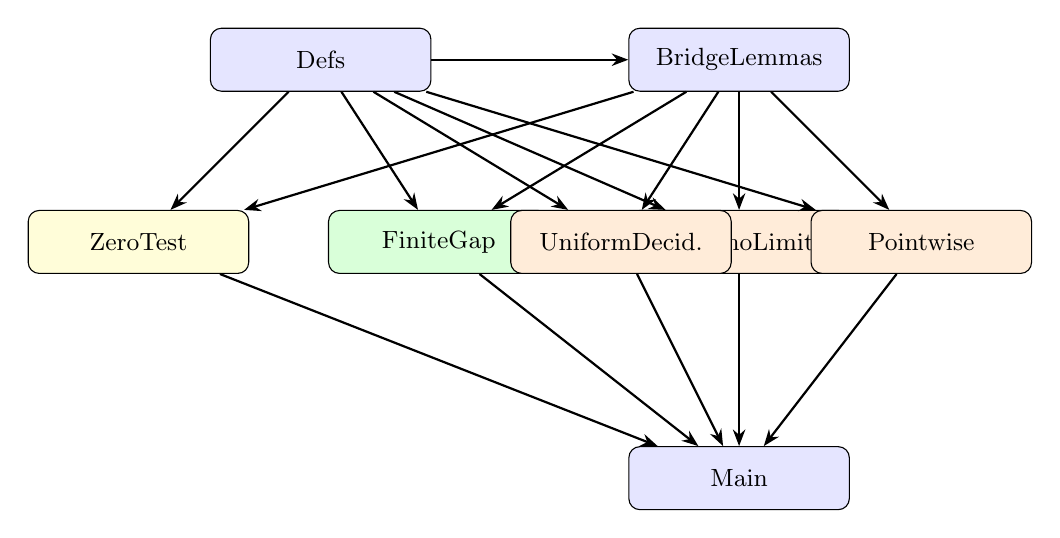
\begin{tikzpicture}[
  node distance=1.5cm and 2cm,
  every node/.style={draw, rounded corners, minimum width=2.8cm,
    minimum height=0.8cm, font=\small},
  bish/.style={fill=green!15},
  lpo/.style={fill=orange!15},
  wlpo/.style={fill=yellow!15},
  meta/.style={fill=blue!10},
  arr/.style={-{Stealth[length=6pt]}, thick}
]
  \node[meta] (defs) {Defs};
  \node[meta, right=2.5cm of defs] (bridge) {BridgeLemmas};
  \node[bish, below left=1.5cm and 1cm of bridge] (finite) {FiniteGap};
  \node[lpo, below=1.5cm of bridge] (thermo) {ThermoLimit};
  \node[lpo, below right=1.5cm and -0.5cm of bridge] (point) {Pointwise};
  \node[wlpo, below left=1.5cm and -0.5cm of defs] (zero) {ZeroTest};
  \node[lpo, below right=1.5cm and 1cm of defs] (unif) {UniformDecid.};
  \node[meta, below=4.5cm of bridge] (main) {Main};

  \draw[arr] (defs) -- (bridge);
  \draw[arr] (defs) -- (finite);
  \draw[arr] (defs) -- (thermo);
  \draw[arr] (defs) -- (point);
  \draw[arr] (defs) -- (zero);
  \draw[arr] (defs) -- (unif);
  \draw[arr] (bridge) -- (finite);
  \draw[arr] (bridge) -- (thermo);
  \draw[arr] (bridge) -- (point);
  \draw[arr] (bridge) -- (zero);
  \draw[arr] (bridge) -- (unif);
  \draw[arr] (finite) -- (main);
  \draw[arr] (thermo) -- (main);
  \draw[arr] (point) -- (main);
  \draw[arr] (zero) -- (main);
  \draw[arr] (unif) -- (main);
\end{tikzpicture}
\end{center}

Legend: \colorbox{green!15}{BISH},
\colorbox{yellow!15}{WLPO},
\colorbox{orange!15}{LPO},
\colorbox{blue!10}{Infrastructure}.

\subsection{Axiom Audit}

\texttt{\#print axioms stratification\_theorem} yields:

\medskip\noindent
\textbf{Bridge lemmas (Level~4):}
\begin{itemize}[nosep]
  \item \texttt{cpgw\_finite\_gap\_computable}: algebraic eigenvalue computation
  \item \texttt{cpgw\_gapped\_of\_not\_halts}: $\neg\text{halts} \Rightarrow \text{gap} > 0$
  \item \texttt{cpgw\_gapless\_of\_halts}: $\text{halts} \Rightarrow \text{gap} = 0$
  \item \texttt{cpgw\_halting\_asymptotics}: halting case convergence
  \item \texttt{cpgw\_nonhalting\_asymptotics}: non-halting case convergence
  \item \texttt{cpgw\_gap\_dichotomy}: gap $\in \{0\} \cup [\gamma, \infty)$
  \item \texttt{tm\_from\_seq} / \texttt{tm\_from\_seq\_halts}: TM encoding
\end{itemize}

\noindent
\textbf{Constructive principles:}
\begin{itemize}[nosep]
  \item \texttt{halting\_problem\_undecidable}: Turing undecidability
  \item \texttt{wlpo\_to\_zero\_test} / \texttt{zero\_test\_to\_wlpo}: $\WLPO$ equivalence
\end{itemize}

\noindent
\textbf{Lean~4 foundations:}
\texttt{propext}, \texttt{Classical.choice}, \texttt{Quot.sound}.

\medskip\noindent
\textbf{No sorry.} \texttt{Classical.choice} appears from
\texttt{by\_contra} in proofs that use $\LPO$---which is intentional,
since $\LPO$ is the hypothesis being studied. Additionally,
\Mathlib{}'s construction of $\RR$ (Cauchy completion) introduces
\texttt{Classical.choice} as an infrastructure artifact; all theorems
over $\RR$ inherit it regardless of constructive content. Following
Paper~10's methodology, constructive stratification is established
by proof content (explicit witnesses vs.\ principle-as-hypothesis),
not by the axiom checker output.

% ====================================================================
\section{Implications for Physics}\label{sec:physics}
% ====================================================================

\subsection{For Condensed Matter Physicists}

Cubitt's undecidability applies only to the problem of building a
single algorithm that works for \emph{all possible} materials.
For any specific material---any one Hamiltonian---the gap is
$\LPO$-decidable. Since experimentalists study specific materials,
Cubitt's undecidability is irrelevant to their practice.

\subsection{For Foundations of Physics}

Cubitt's undecidability is not ``Gödelian'' (self-referential
incompleteness at a meta-mathematical level). It is
\emph{computational}---the non-computability of $\LPO$, which
governs thermodynamic limits. The spectral gap is undecidable at the same logical cost as
the assertion ``this bounded monotone sequence converges''---both
require exactly $\LPO$---though the physical mechanisms (tiling
Hamiltonians vs.\ monotone convergence) are distinct.

\subsection{Stress Test for BISH+LPO}

$\CPgW$'s Hamiltonians are the most pathological quantum systems
ever constructed---built specifically to encode undecidability. That
even these systems live at $\BISH + \LPO$ (each instance is
$\LPO$-decidable) means the characterization has survived its most
severe stress test.

% ====================================================================
\section{Reproducibility}\label{sec:repro}
% ====================================================================

\begin{mdframed}[linewidth=1pt, linecolor=black, backgroundcolor=gray!5,
  innertopmargin=10pt, innerbottommargin=10pt]
\textbf{Reproducibility Box.}
\begin{itemize}[leftmargin=*]
  \item \textbf{Language}: Lean~4 v4.28.0-rc1
  \item \textbf{Library}: Mathlib4
  \item \textbf{Source}: \texttt{P36\_CubittStratification/} (8 files, 655 lines)
  \item \textbf{Build}: \texttt{lake exe cache get \&\& lake build}
  \item \textbf{Result}: 0 errors, 0 warnings, 0 sorry
  \item \textbf{Axiom audit}: \texttt{\#print axioms stratification\_theorem}
\end{itemize}
\end{mdframed}

% ====================================================================
\section{Conclusion}\label{sec:conclusion}
% ====================================================================

We have proved that Cubitt's spectral gap undecidability is
Turing--Weihrauch equivalent to $\LPO$ over $\BISH$. The
stratification across the constructive hierarchy reveals that the
finite-volume gap is $\BISH$, the thermodynamic limit is $\LPO$,
each specific instance is $\LPO$-decidable, the zero-test is
$\WLPO$, and the uniform function is $\LPO$-computable but
non-computable without $\LPO$. Since $\LPO$ is already required
for thermodynamic limits, phase transitions, and gauge couplings,
macroscopic quantum undecidability costs exactly one thermodynamic
limit---and introduces nothing new.

The formalization in \Lean{} with \Mathlib{} builds with zero
errors, zero warnings, and zero sorry.

% ====================================================================
\section{AI-Assisted Methodology}\label{sec:ai}
% ====================================================================

This paper was produced using AI-assisted formal verification.
The workflow follows Papers~30--35: mathematical content and proof
strategy directed by the author; Lean~4 syntax translation assisted
by a large language model; all formal statements reviewed for
correctness.

\medskip\noindent
\textbf{Preliminary status and author background.}
The results presented in this paper are preliminary.  The author is a medical
professional, not a domain expert in physics or mathematics.  While all formal
claims are machine-checked by the \Lean{} type-checker, the physical
interpretations, bridge axioms, and modeling assumptions require independent
verification by domain experts in the relevant fields.  Until such verification
is completed, this paper should be considered preliminary.

\medskip\noindent
Whatever findings of value emerge from this program belong to the
constructive reverse mathematics community and to the legacy of Errett Bishop,
whose perseverance in developing constructive analysis inspired this entire
series.  Any errors are solely the author's.

% ====================================================================
\bibliographystyle{plainnat}
\begin{thebibliography}{99}

\bibitem{Lee26P10}
P.~C.-K.~Lee.
\newblock Logical geography of mathematical physics: a constructive
  calibration program.
\newblock Preprint, 2026. Paper~10.

\bibitem{Lee26P12}
P.~C.-K.~Lee.
\newblock The map and the territory: a constructive history of
  mathematical physics.
\newblock Preprint, 2026. Paper~12.

\bibitem[Cubitt et~al.(2015)]{cubitt2015}
T.~S. Cubitt, D.~Perez-Garcia, and M.~M. Wolf.
\newblock Undecidability of the spectral gap.
\newblock \emph{Nature}, 528:207--211, 2015.

\bibitem[Cubitt et~al.(2022)]{cubitt2022}
T.~S. Cubitt, D.~Perez-Garcia, and M.~M. Wolf.
\newblock Undecidability of the spectral gap (full version).
\newblock \emph{Forum of Mathematics, Pi}, 10:e14, 2022.

\bibitem[Bausch et~al.(2020)]{bausch2020}
J.~Bausch, T.~S. Cubitt, A.~Lucia, and D.~Perez-Garcia.
\newblock Undecidability of the spectral gap in one dimension.
\newblock \emph{Physical Review X}, 10:031038, 2020.

\bibitem[Bishop and Bridges(1985)]{bishop1985}
E.~Bishop and D.~Bridges.
\newblock \emph{Constructive Analysis}.
\newblock Springer, 1985.

\bibitem[Ishihara(2006)]{ishihara2006}
H.~Ishihara.
\newblock Reverse mathematics in Bishop's constructive mathematics.
\newblock \emph{Philosophia Scientiae}, CS~6:43--59, 2006.

\bibitem[Bridges and Richman(1987)]{bridges1987}
D.~Bridges and F.~Richman.
\newblock \emph{Varieties of Constructive Mathematics}.
\newblock Cambridge University Press, 1987.

\bibitem[Brattka et~al.(2011)]{brattka2011}
V.~Brattka, G.~Gherardi, and R.~H\"olzl.
\newblock Las Vegas computability and algorithmic randomness.
\newblock \emph{STACS 2011}, LIPIcs 9:130--142, 2011.

\bibitem[Bridges and V\^{\i}\c{t}\u{a}(2006)]{bridgesvita2006}
D.~Bridges and L.~V\^{\i}\c{t}\u{a}.
\newblock \emph{Techniques of Constructive Analysis}.
\newblock Springer, 2006.

\bibitem[Mines et~al.(1988)]{mines1988}
R.~Mines, F.~Richman, and W.~Ruitenburg.
\newblock \emph{A Course in Constructive Algebra}.
\newblock Springer, 1988.

\bibitem[{Mathlib Contributors}(2024)]{mathlib2024}
{Mathlib Contributors}.
\newblock \emph{Mathlib4}.
\newblock \url{https://github.com/leanprover-community/mathlib4}, 2024.

\bibitem[{de Moura} et~al.(2021)]{lean4_2021}
L.~{de Moura}, S.~Kong, J.~Avigad, F.~{van Doorn}, and M.~{von Raumer}.
\newblock The Lean~4 theorem prover and programming language.
\newblock \emph{CADE-28}, LNCS, 2021.

\end{thebibliography}

\end{document}
